\documentclass{beamer}
\usepackage[utf8]{inputenc}
\usepackage[T1]{fontenc}
\usepackage[english]{babel}
\usepackage{graphicx}
\usepackage{times}
\usepackage{algorithm}
\usepackage{algpseudocode}
\usepackage{amsmath}
\usepackage{amssymb}
\usepackage{tikz}
\usepackage[absolute,overlay]{textpos}

\usetikzlibrary{calc,through,backgrounds,positioning,fit}
\usetikzlibrary{shapes,arrows,shadows,calendar}
\usetheme{Warsaw}
\title{Polska}
\author{Marcin}
\institute{Wydział EAIiIB\\
	Katedra Informatyki Stosowanej}
\date{2019}
\begin{document} 
	\frame{\titlepage}
	
	
	\begin{frame}
	\frametitle{Polska}
	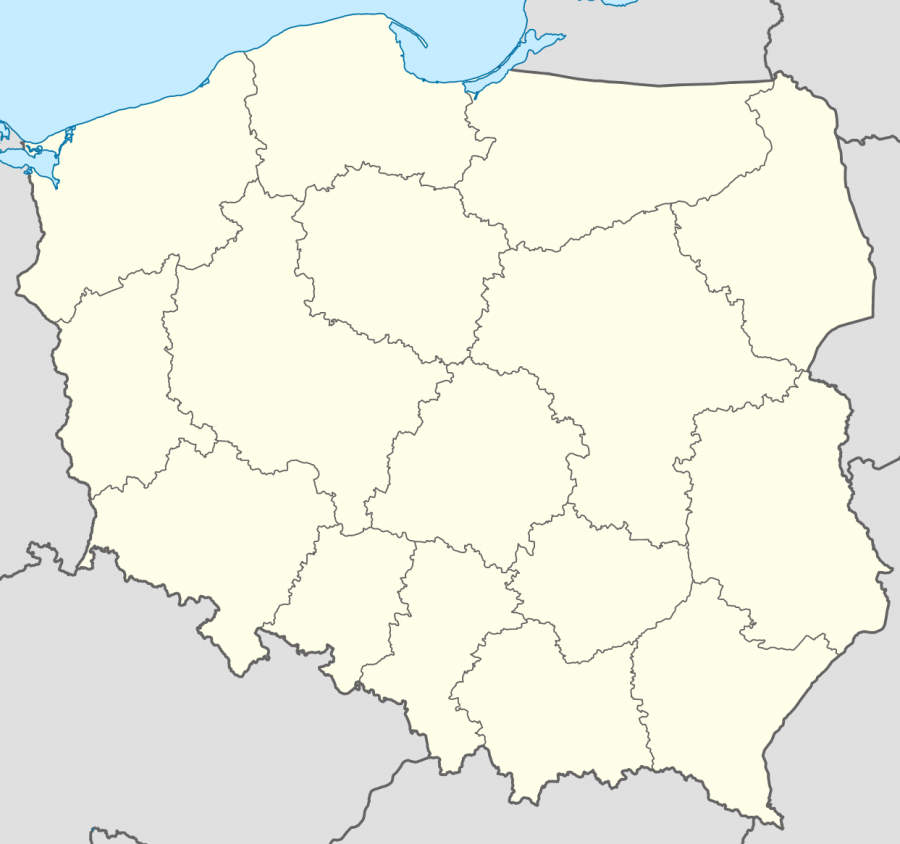
\includegraphics[scale=0.25]{Polska}
\end{frame}

\begin{frame}
\frametitle{Lubelskie}
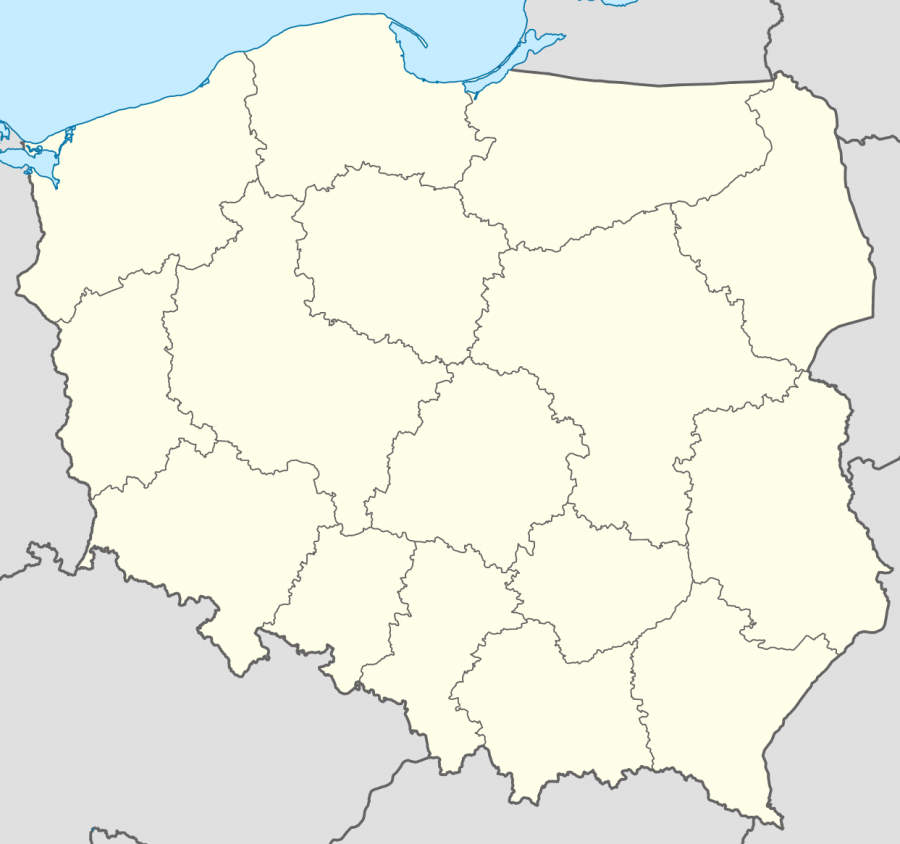
\includegraphics[scale=0.25]{Polska}
\begin{textblock}{3}(8.7,9.3)
	\textcolor{blue}{Lubelskie}
\end{textblock}
\end{frame}

\begin{frame}
\frametitle{Małopolskie}
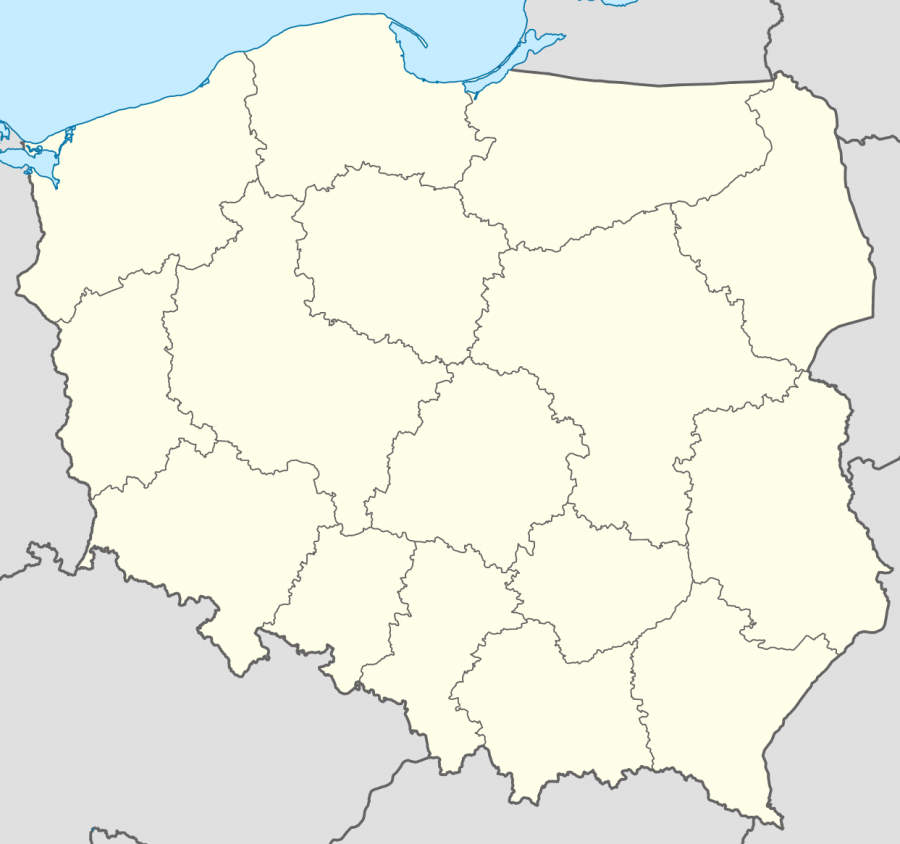
\includegraphics[scale=0.25]{Polska}
\begin{textblock}{3}(8.7,9.3)
\textcolor{blue}{Lubelskie}
\end{textblock}
\begin{textblock}{3}(6.3,12.3)
\textcolor{green}{Małopolskie}
\end{textblock}
\end{frame}

\begin{frame}
\frametitle{Mazowieckie}
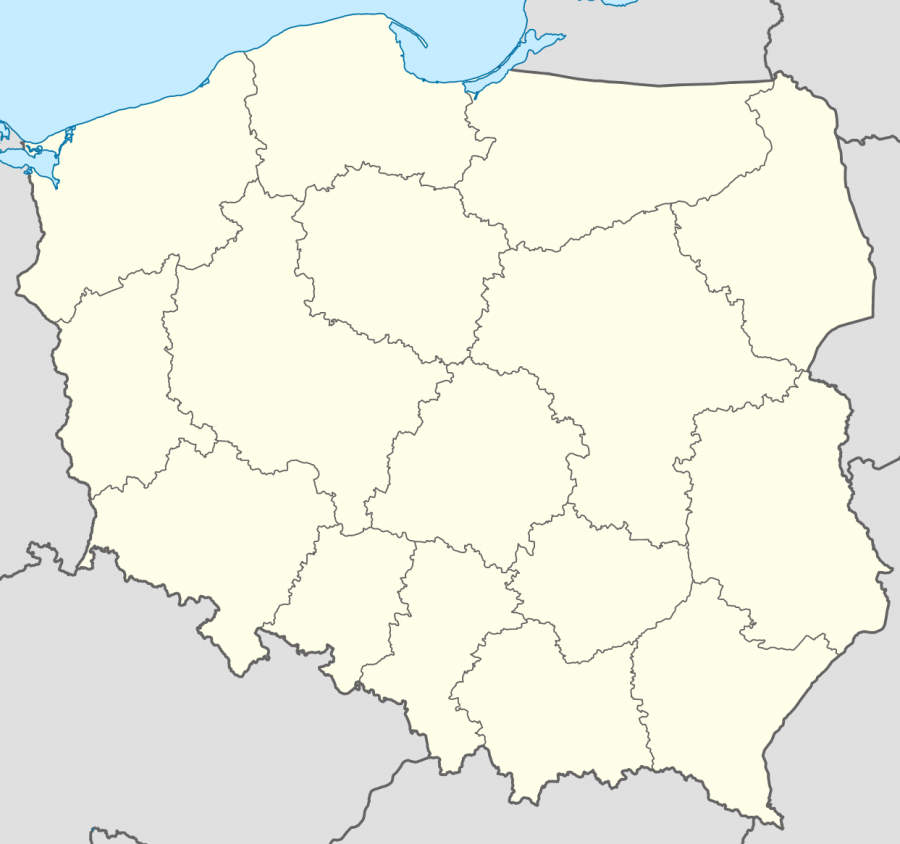
\includegraphics[scale=0.25]{Polska}
\begin{textblock}{3}(8.7,9.3)
\textcolor{blue}{Lubelskie}
\end{textblock}
\begin{textblock}{3}(6.3,12.3)
\textcolor{green}{Małopolskie}
\end{textblock}
\begin{textblock}{3}(7,7)
\textcolor{red}{Mazowieckie}
\end{textblock}
\end{frame}

\begin{frame}
\frametitle{Pomorskie}
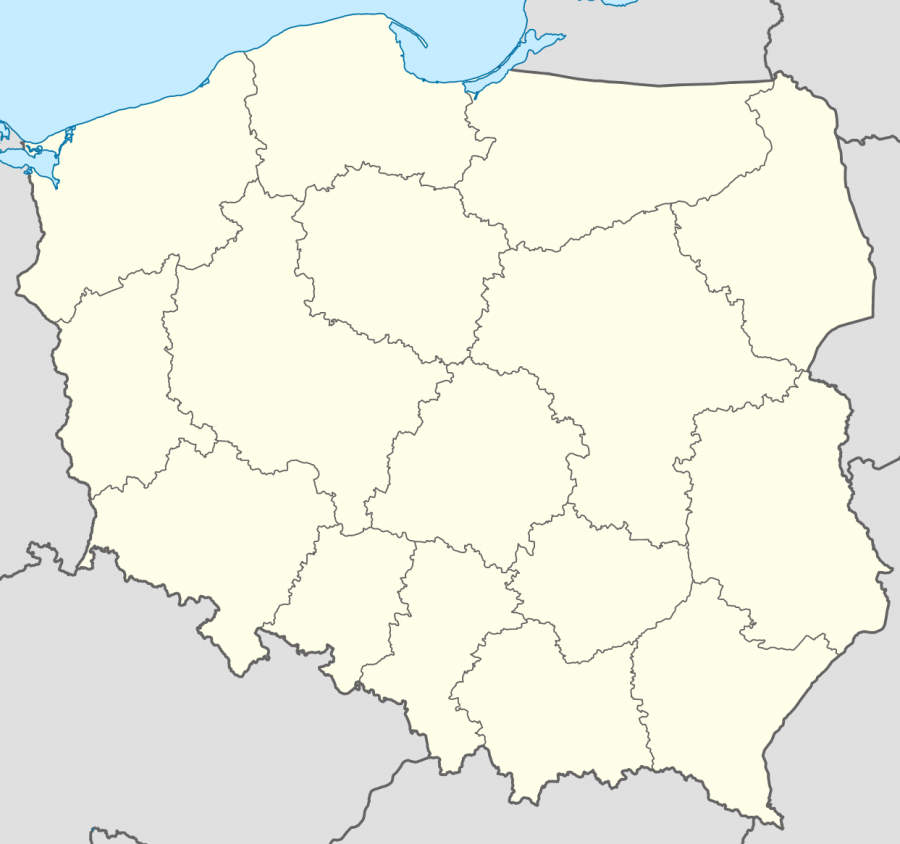
\includegraphics[scale=0.25]{Polska}
\begin{textblock}{3}(8.7,9.3)
\textcolor{blue}{Lubelskie}
\end{textblock}
\begin{textblock}{3}(6.3,12.3)
\textcolor{green}{Małopolskie}
\end{textblock}
\begin{textblock}{3}(7,7)
\textcolor{red}{Mazowieckie}
\end{textblock}
\begin{textblock}{3}(4.1,3.3)
\textcolor{yellow}{Pomorskie}
\end{textblock}
\end{frame}

\begin{frame}
\frametitle{Wielkopolskie}
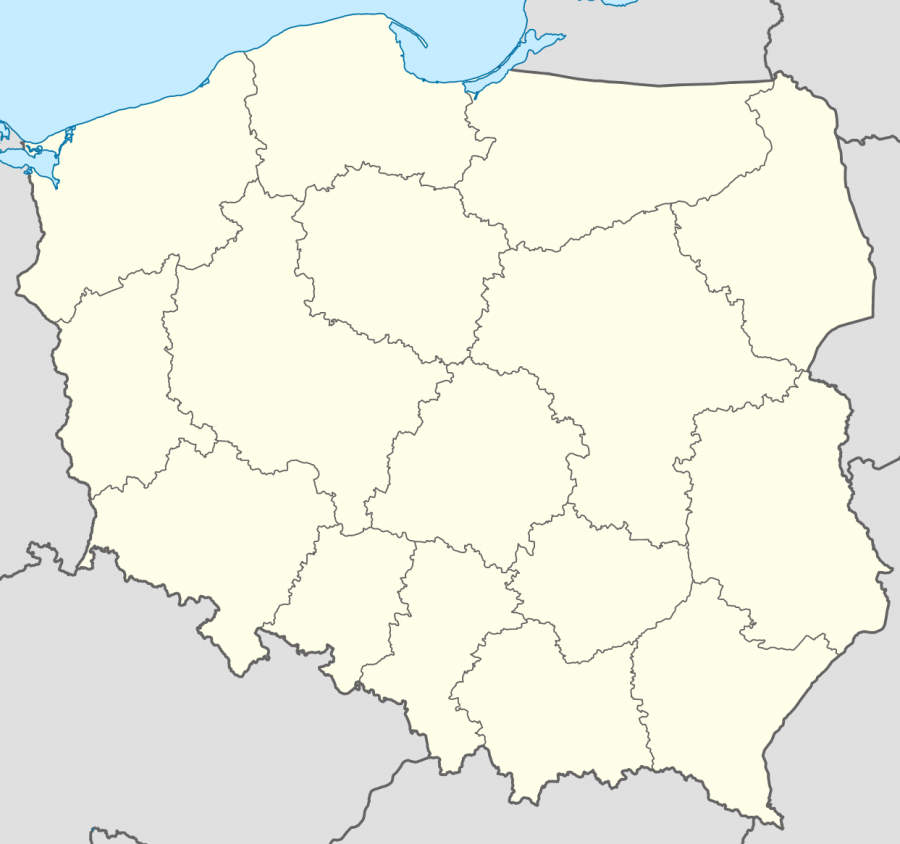
\includegraphics[scale=0.25]{Polska}
\begin{textblock}{3}(8.7,9.3)
\textcolor{blue}{Lubelskie}
\end{textblock}
\begin{textblock}{3}(6.3,12.3)
\textcolor{green}{Małopolskie}
\end{textblock}
\begin{textblock}{3}(7,7)
\textcolor{red}{Mazowieckie}
\end{textblock}
\begin{textblock}{3}(4.1,3.3)
\textcolor{yellow}{Pomorskie}
\end{textblock}
\begin{textblock}{3}(3.2,7)
\textcolor{purple}{Wielkopolskie}
\end{textblock}
\end{frame}
\end{document}